% 獨立 LaTeX 文件：中文、數學、相對圖片、\input 與參考文獻
\documentclass[11pt]{ctexart}
\usepackage{amsmath,amssymb,amsthm}
\usepackage{graphicx}
\usepackage{booktabs}
\usepackage{hyperref}
\graphicspath{{figs/}}
\newtheorem{theorem}{定理}

\title{Mistbox LaTeX 編譯測試}
\author{測試者}
\date{2026 年 11 月}

\begin{document}
\maketitle
\tableofcontents

\section{簡介}
這一節來自 \texttt{sections/intro.tex}，透過 \verb|\input| 引入。


\section{數學環境}
行內公式 $e^{i\pi} + 1 = 0$，以及編號方程式：
\begin{equation}\label{eq:gauss}
  \int_{-\infty}^{\infty} e^{-x^2}\,dx = \sqrt{\pi}
\end{equation}
由式~\eqref{eq:gauss} 可知……
\begin{align}
  (a+b)^2 &= a^2 + 2ab + b^2 \\
  \sum_{k=1}^{n} k &= \frac{n(n+1)}{2}
\end{align}
\begin{theorem}[畢氏定理]
直角三角形中 $a^2 + b^2 = c^2$。
\end{theorem}
矩陣：$\begin{pmatrix} 1 & 2 \\ 3 & 4 \end{pmatrix}$。

\section{圖片與表格}
\begin{figure}[h]
  \centering
  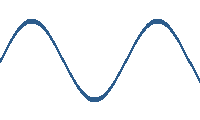
\includegraphics[width=0.4\textwidth]{plot}
  \caption{相對路徑圖片 figs/plot.png}\label{fig:plot}
\end{figure}

\begin{table}[h]
  \centering
  \begin{tabular}{lrr}\toprule
  項目 & 數量 & 單價 \\\midrule
  咖啡 & 2 & 80 \\
  蛋糕 & 1 & 120 \\\bottomrule
  \end{tabular}
  \caption{表格}
\end{table}

見圖~\ref{fig:plot} 與文獻~\cite{knuth1984}。

\bibliographystyle{plain}
\bibliography{refs}
\end{document}
